In this chapter, the concepts required to better understand this thesis are briefly described. Section \ref{section:Parameter estimation} describes the parameter estimation problem and explains estimation of parameters on incomplete data using the Expectation Maximization algorithm. Section \ref{section:conjugate priors} explains the conjugate priors for binomial distribution and generalizes it to a Multinomial distribution. The final section \ref{section:topic modelling} describes the topic models, Probabilistic Latent Semantic Analysis (PLSA) and Probabilistic Latent Sequential Motifs (PLSM).
\section{Parameter estimation} 
\label{section:Parameter estimation}
Parameter estimation \cite{Heinrich04parameterestimation} is the problem of finding the parameters $\theta$ for a set of distributions that best explains the observations $X$. 
The dataset $X$ $=\{x_{i}\}_{i=1}^{|X|}$ can be considered as a set of observations generated independently and identically distributed realizations of a random variable. The parameters $\theta$, depends on the distributions considered, for example, Multinomial distribution, $\theta$ $= \{p_{i}\}_{i=1}^{i=D}$, where D is the cardinality of the possible outcomes.

The joint distribution $P(X,\theta)$ describes the probability of the observations for different combinations of the vector $\theta$. Bayes theorem gives the relationship between the probabilities $X$ and $\theta$ as below:
\begin{equation}
\label{equ:bayes}
P(\theta|X) = \frac{P(X|\theta) P(\theta)}{P(X)} 
\end{equation}
The interpretation of the distributions in Eq. \ref{equ:bayes} is given below:
\begin{equation}
posterior ~\alpha \ liklihood \times prior
\end{equation}
Below, we explain some of the methods for parameter estimation. We will start with simple Maximum Liklihood Estimation (MLE) and then describe how prior belief can be included in the estimation. 

\subsection{MLE}
\label{section:MLE}
MLE is the method of finding the parameters of the model that maximizes the probability of the observations(liklihood) under the resulting distribution. The liklihood is,
\begin{equation}
\ell(\theta|X) = \prod _{i=1}^{i=|X|} P(x_{i}|\theta)
\end{equation}
Because of the product, it is often mathematically convenient to express the liklihood, $\ell$, as the log-liklihood,
\begin{equation}
L(\theta|X) = \sum_{i=1}^{i=|X|} log(P(x_{i}|\theta))
\end{equation}
The MLE can then be formulated as,
\begin{equation}
\label{equ:log-liklihood}
\theta_{ML} = \arg \! \max_\theta(L(\theta|X))
\end{equation}

The parameter $\theta$ then can be estimated by solving the Eq. \ref{equ:log-liklihood} as follows:
\begin{equation}
\frac{\partial}{\partial\theta_{d}} L(\theta|X) = 0; \forall \theta_{d} \in \theta
\end{equation}
As an example, consider a set $X$ of $N$ bernoulli experiments of an unfair coin toss with unknown parameter $\theta$. The probability of the event $c$, for a single experiment, for the random variable(r.v) $C$ is,
\begin{equation}
P(X=x|\theta) = \theta^{x}\cdot\theta^{1-x} 
\end{equation}
where $x=1$ is heads and $x=0$ is tails.
The MLE for $\theta$ can be found by solving Eq. \ref{equ:log-liklihood},
\begin{eqnarray}
L & = & \sum_{i=1}^{i=N}(log(P(X=x|\theta))) \\
 & = & (n^{1}log(P(X=1|\theta))) + n^{0}log(P(X=0|\theta)))
\end{eqnarray}
where $n^{1}$ denotes the number of heads and $n^{0}$, the number of tails.
\begin{equation}
\frac{\partial}{\partial\theta}(L) = \frac{x^{1}}{\theta} - \frac{x^{0}}{1-\theta}=0 
\end{equation}
\begin{equation}
\label{equ:ML}
\theta_{ML} = \frac{x^{1}}{x^{1}+x^{0}} = \frac{x^{1}}{N} 
\end{equation}
which is the ratio of heads to the total number of samples. 

It can be seen from Eq. \ref{equ:ML}, the MLE estimates parameters which best explains the observations. If the observations or the sample dataset(subset of sample space) is not a good representative of the population(sample sapce) then the MLE estimate approach overfits the parameters to the sample dataset.

\subsection{Maximum a posteriori estimation}
Maximum a posteriori (MAP) estimation is similar to MLE but also incorporates a mechanism to add prior belief in the form of a prior distribution. In MAP, the parameters of the model are obtained by maximizing the posterior distribution in Eq. \ref{equ:bayes} with respect to the model parameters $\theta$
\begin{eqnarray}
\theta_{MAP} & = & \arg\!\max_\theta(P(X|\theta) \cdot P(\theta)) \ \ \ \ \mid \scalebox{0.75}{$ P(X) \neq f(\theta)$} \\
& = & \arg\!\max_\theta(\sum_{i=1}^{N}log(P(x_{i}|\theta)) + log(P(\theta)))
\label{equ:MAP}
\end{eqnarray}
Continuing with the coin example as in MLE, the prior distribution $P(\theta)$ is represented by the Beta distribution(explained in Section \ref{section:conjugate priors}) with hyperparameters $\alpha$ and $\beta$ as below:
\begin{eqnarray}
P(\theta) & = & \frac{\theta^{\alpha}\cdot(1-\theta)^{\beta}}{B(\alpha,\beta)} \ \ \ \ \mid \scalebox{0.75}{$B(\alpha,\beta)$ = beta function}
\end{eqnarray}
\begin{equation}
\label{equ:prior}
\frac{\partial}{\partial\theta}P(\theta) = \frac{\alpha-1}{\theta} + \frac{\beta-1}{\theta}
\end{equation}
Substituting Eq. \ref{equ:ML} and \ref{equ:prior} in \ref{equ:MAP} and simplifying, we obtain,
\begin{equation}
\label{equ:MAP estimate}
\theta_{MAP} = \frac{x^{1}+\alpha-1}{N+\alpha-1+\beta-1}
\end{equation}
From the MAP estimate in Eq. \ref{equ:MAP estimate}, we can see that, the addition of prior distribution is just including past experimental results or belief.
The addition of prior belief acts like regularization to the MLE estimate
\section{EM algorithm}
Expectation Maximization(EM) algorithm is an iterative approach for parameter estimation for incomplete dataset. The missing values in the data corresponds to unobserved variables which are also know as hidden or latent variables. Each iteration of the EM algorithm consists of two steps: The E-step and the M-step. In the E-step, the missing data is estimated with the current estimate of the parameters. In the M-step, the liklihood function is maximized based on the estimate obtained in the E-step for the missing data.
Consider a set $X$ of observed data, a set $Z$ of unobserved data and $\theta$ be a vector of unknow model parameters. The log-liklihood of the observed data is given below:
\begin{equation}
\label{eqn:EM-likli}
L(\theta|X) = \sum_{z}P(X|z,\theta)P(z|\theta)
\end{equation}
As explained previously, EM algorithm iteratively maximizes $L(\theta|X)$. Assume that after the $n^{th}$ iteration the parameters are $\theta_{n}$. Since the objective is to maximize Eq \ref{eqn:EM-likli}, the updated estimate for the model parameters $\theta$ should satisfy,
$L(\theta)$ $\geq$ $L(\theta_{n})$
Equivalently, we can maximize the difference:
\begin{equation}
\label{equ:diff}
L(\theta) - L(\theta_{n})= \Delta(\theta|\theta_{n}) = log(P(X|\theta)) - log(P(X|\theta_{n}))
\end{equation}
Simplifying \ref{equ:diff} we get:
\begin{equation}
\Delta(\theta|\theta_{n}) = \sum_{z}P(z|X,\theta)log(P(z|X,\theta_{n})\cdot P(X|\theta_{n}))
\end{equation}
\begin{equation}
L(\theta) \geq \Delta(\theta|\theta_{n}) + L(\theta_{n})
\end{equation}
For convenience let:
\begin{equation}
Q(\theta|\theta_{n}) = \Delta(\theta |\theta_{n}) + L(\theta_{n})
\end{equation}
The function $Q(\theta|\theta_{n})$ called Q-function, is bounded by the liklihood $L(\theta)$. Our objective is to choose $\theta$ that maximizes the Q-function. Any $\theta$ that maximizes the Q-function also maximizes $L(\theta)$. We denote this updated value of $\theta$ as $\theta_{n+1}$
\begin{align*}
\label{equ:EM_algo}
\theta_{n+1} & =  \arg\max_{\theta}(Q(\theta|\theta_{n})) \\
 & =  \arg\max_{\theta}(\sum_{z}P(z|X,\theta)\cdot P(X,z|\theta))) \addtag
\end{align*}
Thus from Eq. \ref{equ:EM_algo} the steps of the EM algorithm are evident. The following steps are iterated untill convergence:
\begin{enumerate}
\item E-step: Calculate the conditional expectation $\sum_{z}P(z|X,\theta)\cdot P(X,z|\theta))$
\item M-step: Maximize Eq. \ref{equ:EM_algo} with respect to $\theta$
\end{enumerate}

 
\section{Conjugate Priors} 
In Section \ref{section:MLE} it was shown that the MLE estimate leads to overfitting the parameters if the sample dataset is not a good representation of the population. The MAP estimate overcomes this problem by introducing a prior distribution $P(\theta)$ over the parameter $\theta$. The prior distribution is choosen such that, it has simple interpretation and useful analytical properties. The posterior distribution is proportional to the product of liklihood and prior. If the posterior and prior have same functional form then they are know as conjugate pairs. 

\subsection{Beta distribution}
The beta distribution is a continuos distribution in the interval $[0,1]$ parameterized by two positive shape parameters $a,b$.
\begin{equation}
Beta(\theta|a,b) = \frac{\Gamma(a+b)}{\Gamma(a) \Gamma(b)} \cdot \theta^{a-1} (1-\theta)^{b-1}
\end{equation}
The parameters $a$ and $b$ are also called hyperparameters because they control the distribution of the $\theta$ parameter. The varaince of the beta distribution is governed by the value of the hyperparameters as illustrated in Fig  The beta distribution has similar form as the binomial distribution.  The liklihood function in case of a dataset sampled from a binary random variable takes the form $\theta^{l}(1-\theta)^{m}$. By using the beta distribution as prior, the posterior can then be calulated using the Baye's rule in \ref{equ:bayes}.
\begin{figure}
\begin{center}
\includegraphics{betaDistribution.jpg}
\caption{Beta Distribution: Depicts the variance of beta distribution for various hyperparameters}
\end{center}
\end{figure}

\begin{equation}
\label{eqn:beta}
posterior(\theta|l,m,a,b) = \frac{\Gamma(a+b+l+m)}{\Gamma(a+l) \Gamma(b+m)} \theta^{a+l-1} (1-\theta)^{b+m-1} = Beta(\theta|a+l,b+m) 
\end{equation}

As seen from Eq. \ref{eqn:beta}, the posterior distribution takes the form of the beta distribution. 

\subsection{Dirichlet distribution}
In case of a Multinomial liklihood function, the beta distribution can be generalized from 2 to K dimensions.
\begin{equation}
Dir(\vec{\theta}|\vec{\alpha}) = \frac{\Gamma(\sum_{k=1}^{K}\alpha_{k})}{\prod_{k=1}^{K}\Gamma(\alpha_{k})}\prod_{k=1}^{K}\theta_{k}
\end{equation}
Similar to the Beta distribution, the posterior distribution in case of Multinomial liklihood function can be shown to the take form of a Dirichlet distribution.
\label{section:conjugate priors}
\section{Topic modelling}
\label{section:topic modelling}
Topic models ~\cite{steyvers2006probabilistic,blei2011introduction} are a suite of algorithms that aim at expressing documents as a mixture of topics. A topic is a distribution over words. Topic models are generative models, A document is generated by first choosing a distribution over topics, then randomly choosing a topic from this distribution and draw a word from that topic. Using standard inference techniques the parameters for the distributions can be infered. In this chapter we will be descussing Probabilistic Latent Semantic Analysis (PLSA) and Probabilistic Latent Sequential Motifs (PLSM). These models do not make any assumptions about the order of the words in the document. This is know as the bag of words approach to modeling text.

\subsection{PLSA}
Latent semantic analysis (LSA) represents documents in a lower dimensional space called the latent semantic space by linear projection of term-document matrix through singular value decomposition. The term-document matrix represents the frequency of words from a pre defined vocbulary in a document. LSA has deficits like, capturing polysems and interpretation is difficult due to its unsatisfactory statiscal foundation. Probabilistic Latent Semantic Analysis (PLSA) introduces a statiscal foundation to LSA, since it is based on a liklihood principle and defines a generative model of document pertaining to the dataset ~\citep{Hofmann99probabilisticlatent}.

\begin{wrapfigure}{r}{0.40\textwidth}
\label{PLSM-genModel}
 \vspace{-20pt}
\begin{center}

\includegraphics[width=0.38\textwidth]{PLSA}
\end{center}
 \vspace{-10pt}
 \caption{PLSA generative model: $d$ is the document variable, $z$ is the topic variable dependent on $d$ and $w$ is the word variable independent of $d$ given $z$. $d$ and $w$ are observed variables. $N_{d}$ is the document length and $M$ is the number of documents}
\vspace{-10pt}
\end{wrapfigure}
PLSA adopts the aspect model to model the joint probability of each co-occurrence of a word $ w ~\epsilon \ W = \{w_{1},w_{2}, \cdots , w_{V}\}$($V$ is the size of the vocabulary) in a document $ d ~\epsilon \ D = \{d_{1},d_{2}, \cdots , d_{M}\}$ by associating a latent class variable $z$. The generative process of the model in Fig. \ref{PLSM-genModel}  can be explained as below :

\begin{itemize}
\item[$\cdot$] pick a document $d$ with probability $P(d)$.
\item[$\cdot$] pick a topic with probability $P(z|d)$
\item[$\cdot$] pick a word from topic $z$ with probability $P(w|z)$
\end{itemize}

The above description joint probability model of PLSA is given by the expression:
\begin{eqnarray}
P(w,d) & = & P(d)\cdot P(w|d) \\
P(w|d) &= & \sum_{z}P(w|z)P(z|d)
\end{eqnarray}
PLSA is a mixture model. This is based upon the conditional independence assumption that given a topic, the choice of word is independent of the document. 

The parameters $P(z|d)$, $P(w|z)$ and $P(d)$ can be estimated by maximizing the log-liklihood function using the EM algorithm.
\begin{equation}
L = \sum_{d}\sum_{w}n(w,d)log(P(w,d)).
\end{equation}

The E-step can be obtained by using Baye's rule:
\begin{equation}
P(z|d,w) = \frac{P(z|d)\cdot P(w|z)}{\sum_{z}P(z|d)\cdot P(w|z)}
\end{equation}

By standard calculations, the equations for M-step can be obtained:
\begin{eqnarray}
P(z|d) & = & \frac{\sum_{w} n(w,d)P(z|w,d)}{\sum_{w}\sum_{z^{'}}n(w,d)P(z^{'}|w,d)} \\
P(w|z) & = & \frac{\sum_{d} n(w,d)P(z|w,d)}{\sum_{w}\sum_{d}n(w^{'},d)P(z|w{'},d)} \\
P(d) & = & \frac{\sum_{z}\sum_{w} n(w,d)P(z|w,d)}{\sum_{d^{'}}\sum_{w}\sum_{z}n(w,d^{'})P(z|w,d^{'})}
\end{eqnarray}





\subsection{PLSM}
Topic models like PLSA and LDA have been shown successful in capturing scene level activity patterns by co-occurrence analysis of low level features (words). These models fail to capture the temporal order of co-occurence of words. These topic models have been adapted (like HMM on top of LDA) ~\cite{} to discover temporal patterns but have drawbacks discussed here ~\cite{Varadarajan_IJCV_2012,varadarajan_probabilistic_2010}. Probabilistic latent sequential motifs(PLSM) ~\cite{Varadarajan_IJCV_2012,varadarajan_probabilistic_2010} addresses some of these drawbacks by capturing spatio-temporal co-occurences of words in a temporal window called motifs and the starting time of occurence of these motifs. 

\begin{wrapfigure}{r}{0.30\textwidth}
\label{fig:PLSM}
 \vspace{-20pt}
\begin{center}
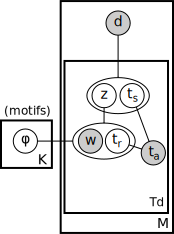
\includegraphics[width=0.38\textwidth]{PLSM}
\end{center}
 \vspace{-10pt}
 \caption{PLSM generative model: $d$ is the document variable, $z$ is the topic variable dependent on $d$ and $w$ is the word variable independent of $d$ given $z$. $d$ and $w$ are observed variables. $Td$ is the document length and $M$ is the number of documents}
\vspace{-10pt}
\end{wrapfigure}

Figure. \ref{fig:PLSM} shows the generative process of PLSM. Let $D = \{d_{1},d_{2},d_{3}, \cdots, d_{M}\}$ represent the set of documents (like videos from a surveillance camera), $W = \{w_{1},w_{2}, \cdots, w_{V}\}$ represents the vocabulary, $Ta = \{t_{1},t_{2}, \cdots, t_{Td}\}$ represents the time of occurrence of words in the document $d$. Then according to our model, the documents can be described by a set of motifs $Z=\{z_{1}, z_{2}, \cdots, z_{K}\}$ which have a duration of $Tz$ i.e $tr = \{t_{1}, t_{2}, \cdots, t_{Tz}\}$. Each motif can occur at any time $ts = \{t_{1}, t_{2}, \cdots, t_{Tds}\}$ in a document $d$. The generative process of the PLSM model can be described as follows:
\begin{itemize}

\item[$\cdot$] Pick a document $d$ from $P(d)$
\item[$\cdot$] Pick topic $z$ and it's starting time $ts$ from $P(z,ts|d)$
\item[$\cdot$] Pick a word $w$ and relative time $tr$ from $P(w,tr|z)$ 
\item[$\cdot$] Set ta=ts+tr or equivalently $P(ta|ts,tr)$ is a Dirac function at ta

\end{itemize}
The joint probability distribution $P(w,ta,d,z,ts,tr)$ can be obtained from the model as below:
\begin{eqnarray}
P(w,ta,d,z,ts,tr) & = & P(d)P(z,ts|d)P(w,tr|z)P(ta|tr,ts) \\
				 & = &\begin{cases}
    P(w,z,ts,tr,d),& \text{if } ta = ts+tr\\
    0,              & \text{otherwise}
\end{cases}
\end{eqnarray}

Given a corpus of documents $C$ in the form of term frequency matrix $n(w,ta,d)$, the liklihood of the data is given by the expression:
\begin{equation}
P(C) = \prod_{w,ta,d} P(w,ta,d)^{n(w,ta,d)}
\end{equation}

The motifs $P(w,tr|z)$ and their start times $P(z,ts|d)$ which form the parameters of the model can be infered from the observations. The inference is performed by maximizing the log-liklihood of the data. The inference is also guided towards estimating a sparse distribution of $P(z,ts|d)$ which is motivated in ~\cite{Varadarajan_IJCV_2012,varadarajan_probabilistic_2010}.
\begin{equation}
L(D|\theta) = \sum_{w,ts,tr,d} n(w,ts+tr,d)log(\sum_{z,ts} P(w,tr,d,z,ts)) + KL(U||P(z,ts|d))
\end{equation}
 Since the data is paratially observed, parameters are estimated using the expectation maximization algorithm.
 \begin{equation}
 E[L] = \sum_{w,ts,tr,z,d}n(w,ts+tr,d)P(z,ts|w,ts+tr,d)log(P(w,ts+tr,d,z,ts)) - \sum_{z,ts,d}\frac{\lambda_{d}}{K \cdot Tds} log(P(z,ts|d))
 \end{equation}
 
 The E-Step can be obtained Baye's rule
 \begin{equation}
 P(z,ts|w,ta,d) = \frac{P(z,ts|d)P(w,tr|z)}{\sum_{z,ts}P(z,ts|d)P(w,tr|z)}
 \end{equation}

The M-step expressions can be obtaiend by standard calculations
\begin{eqnarray}
P(z,ts|d) & \alpha & max(\epsilon, \sum_{w,tr}n(w,ts+tr,d)P(z,ts|w,ts+tr,d)- \frac{\alpha_{d}}{K\cdot Tds}) \\
P(w,tr|z) & \alpha & \sum_{ts,d}n(w,ts+tr,d)P(z,ts|w,ts+tr,d)
\end{eqnarray}

The term $\lambda_{d}$ as in ~\cite{Varadarajan_IJCV_2012,varadarajan_probabilistic_2010} is defined as $\lambda$$nd$ where nd is the number of words in the document $d$ and $\lambda$ indicates the sparsity level.

